\chapter{Medical Fundamentals}
Comprehension of the physiological functionality of the human heart and the cardiovascular system is an important prerequisite to the work addressed in this thesis. Therefore the basics of these topics will be explained in this chapter.

\section{Cardiovascular System}
The fundamental task of the cardiovascular system is to supply all organs with blood. The system is divided into two components. The systemic circulation and the pulmonary circulation. As shown in \figurename~ \ref{fig:circulation}, which represents the percentage distribution of the blood over the circulatory system, the systemic circulation is supplying blood flow to all tissues and organs except the lung. Due to this, it is also referred to as the greater circulation. \cite{GH20}
\begin{figure}[h]
  \centering
  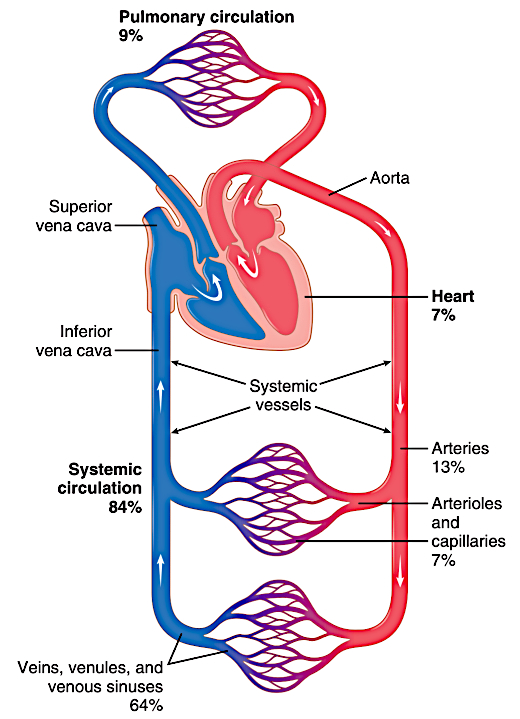
\includegraphics[width=0.4\textwidth, height=0.6\textwidth]{images/circulation.jpg}
  \caption{Blood distribution in the circulatory system \cite{GH20}.}
  \label{fig:circulation}
\end{figure}
 \\The center of the cardiovascular system is the heart. The heart itself consists of two mechanical pumps, which are functionally connected in series but are united in one organ. It is separated into two sides, which themselves are divided into an atrium and a ventricle each. The atria act as weak primer pumps needed to provide blood flow to the ventricles.\cite{HKS4} Both, the atria and the ventricles are surrounded by the myocardium, which acts as the working muscle of the heart. Through the contraction of the myocardium, blood is pumped into the circulatory system.\cite{HKS7} The left ventricle is pumping oxygenated blood through the aorta into the systemic circulation. There, the oxygen stored in the blood is delivered to the organs. The blood, now low in oxygen, is then led into the right atrium through the inferior and superior vena cava. From the right atrium, the deoxygenated blood then enters the right ventricle and afterwards is directed into the pulmonary circulation via the pulmonary artery. After the blood is oxygenated in the lungs, it is returned to the left atrium through the pulmonary vein.\cite{HKS4} In addition to the atria and the ventricles each side of the heart has an atrioventricular (A-V) valve, as well as a semilunar (SL) valve. The A-V valve of the left heart is called the mitral valve, the one of the right heart is referred to as the tricuspid valve. The aortic valve and pulmonary valve are the SL valves of the left and right heart, respectively.\cite{HKS7} \figurename~ \ref{fig:heart_anat} provides a graphic overview of the anatomy of the heart and the course of blood flow through the heart.

 \begin{figure}[h]
   \centering
   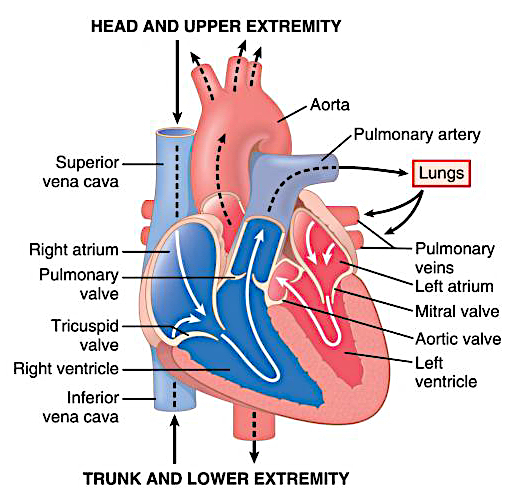
\includegraphics[width=0.6\textwidth]{images/heart_1.jpg}
   \caption{Anatomy of the human heart \cite{GH20}.}
   \label{fig:heart_anat}
 \end{figure}
 %\\
 The amount of blood pumped through the two sides of the heart is equal at all times. This value is called cardiac output (CO). It is calculated through by multiplying the heart rate (HR) and the stroke volume (SV). For an average adult at rest, with a heart rate of approximately $70 min^{-1}$ and a stroke volume of 70 ml, this leads to
 \begin{equation}
   CO = HR \times SV = 70 min^{-1} \times 70ml = 5 \frac{l}{min}
  \label{eq:CO}
 \end{equation}
In case of maximum physical load, the cardiac output can increase as high as $20\frac{l}{min}$, for a stroke volume of 110 ml and a heart rate of $190 min^{-1}$. \cite{HKS4}

The cardiac cycle describes the events that occur during the time-span of one heartbeat. It is triggered by an electrochemical action potential originating from the sinus node. The cycle is divided into four phases. \figurename~ \ref{fig:cardiac_cycle} illustrates these action phases and events of the cardiac cycle for the left ventricle.
\begin{figure}[h]
  \centering
  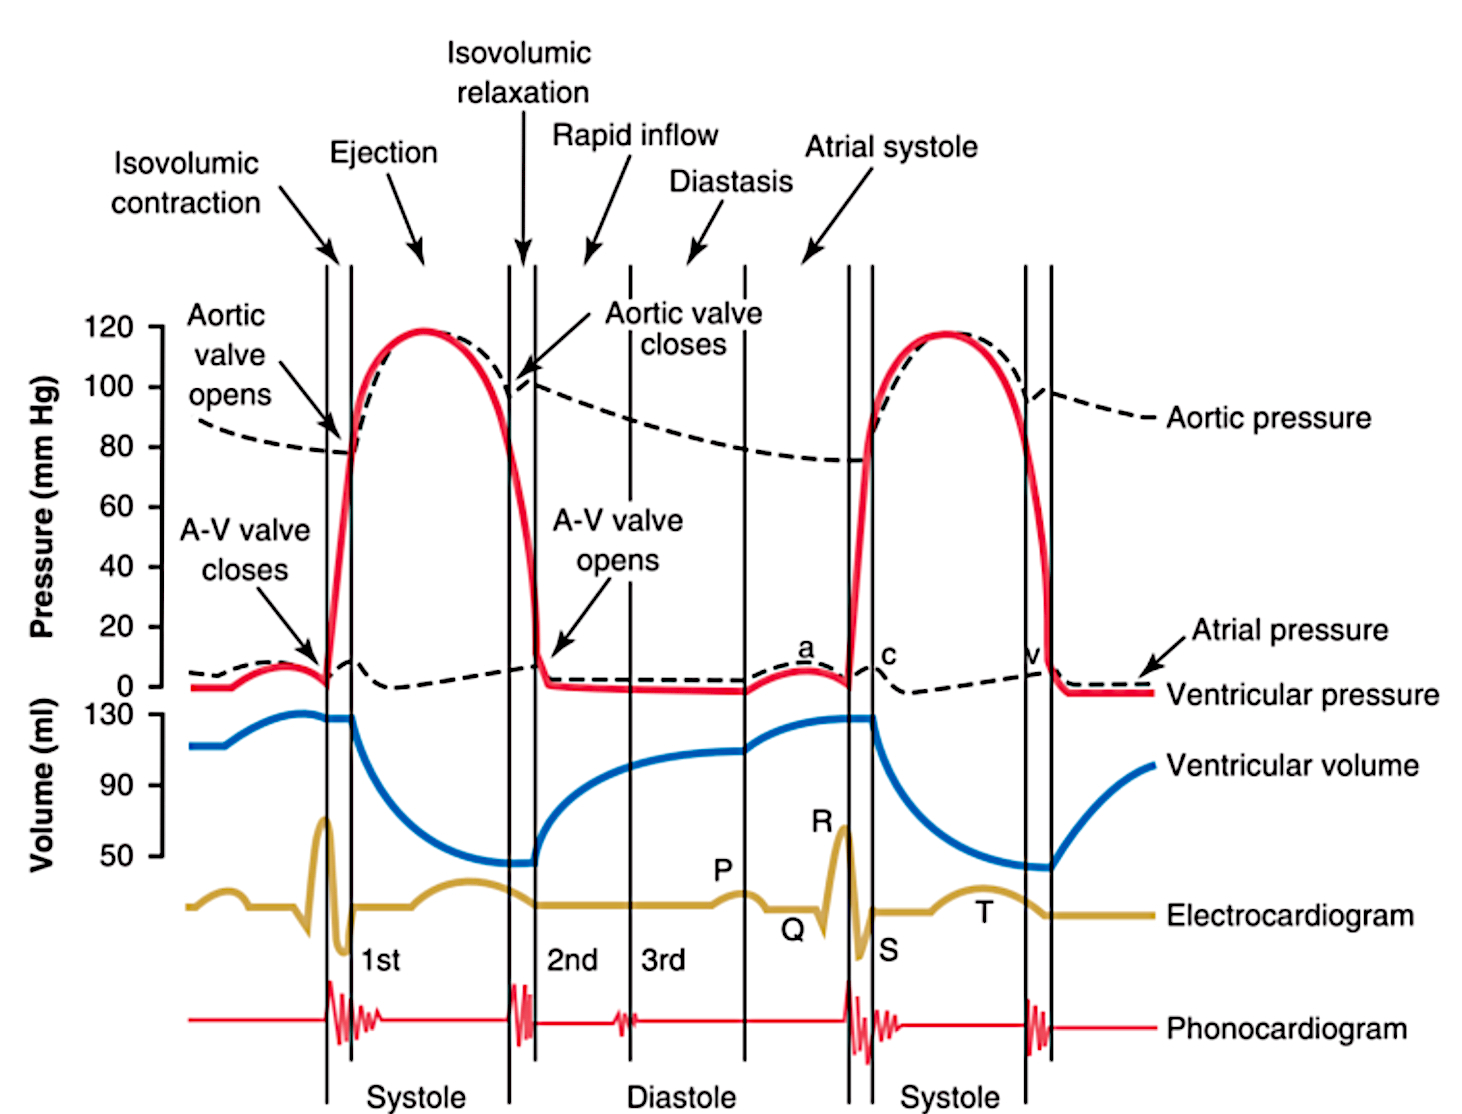
\includegraphics[width=0.8\textwidth]{images/cardiac_cycle.jpg}
  \caption{Action phases of the cardiac cycle based on the example of the left ventricle \cite{GH20}.}
  \label{fig:cardiac_cycle}
\end{figure}
During the period of isovolumic contraction, the ventricular pressure increases. For the left ventricle, the pressure increases from about 4-6 mmHg to 80 mmHg. The values for the right ventricle are much lower. This increase is happening as a direct result of the ventricular contraction. The A-V valves, as well as the SL valves, are closed during this process. This leads to a constant blood volume in the ventricles. As soon as the ventricular pressure exceeds the arterial pressure the pulmonary and aortic valves open and blood can flow into the aorta and the pulmonary artery. This phase is called ejection phase, as the blood is ejected into the circulatory system. The period of isovolumic contraction in combination with the ejection phase is called systole.\cite{HKS4} During the systole the blood volume in the ventricle decreases by 55-60\%, resulting in an end-systolic volume (ESV) of about 40-50 ml \cite{GH20}. Due to the contraction of the myocardium, the ventricular pressure keeps increasing for a while before decreasing again as the relaxation of the myocardium sets in. As soon as the outflow of the blood ends, the semilunar valves close, initiating the period of isovolumic relaxation. During this period pressure in the ventricles is decreasing, while the blood volume is constant. When the pressure in the atrium exceeds the ventricular pressure, the A-V valves open and blood is flowing into the ventricles until the pressure levels are balanced.\cite{HKS4} This phase is referred to as the period of rapid filling of the ventricles. Combined with the isovolumic relaxation it represents the diastole. The end-diastolic volume (EDV) is about 110-120 ml.\cite{GH20} While, at rest, the diastole lasts about twice as long as the systole, above a heart rate of 150$min^{-1}$, the two phases are about equal \cite{HKS4}.

%\\
The pumping mechanism of the left ventricle can be illustrated well using a pressure-volume diagram (P-V diagram). For the construction of the P-V diagram first the relationship between the left ventricular volume and the ventricular pressure during diastole and systole, as displayed in \figurename~\ref{fig:pv_1}, has to be discussed.
\begin{figure}[h]
  \subfloat[]
  {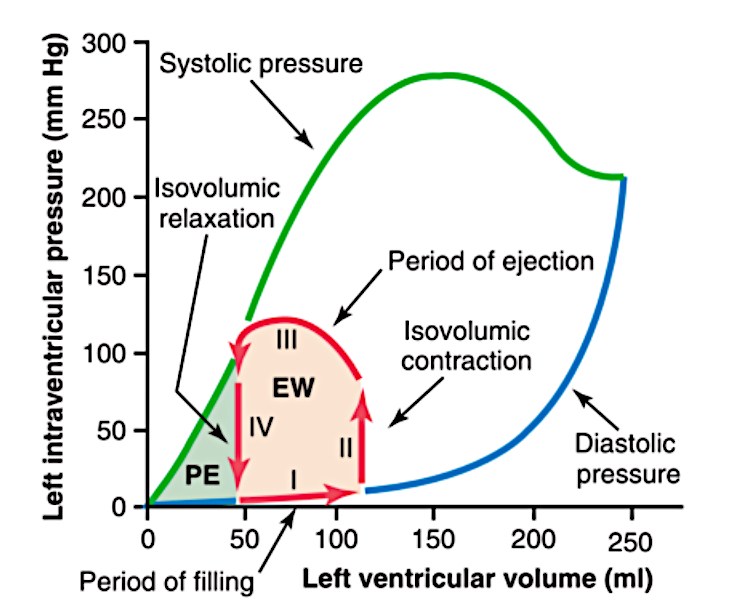
\includegraphics[width=0.5\textwidth]{images/pv_1.jpg}\label{fig:pv_1}}
  \subfloat[]
  {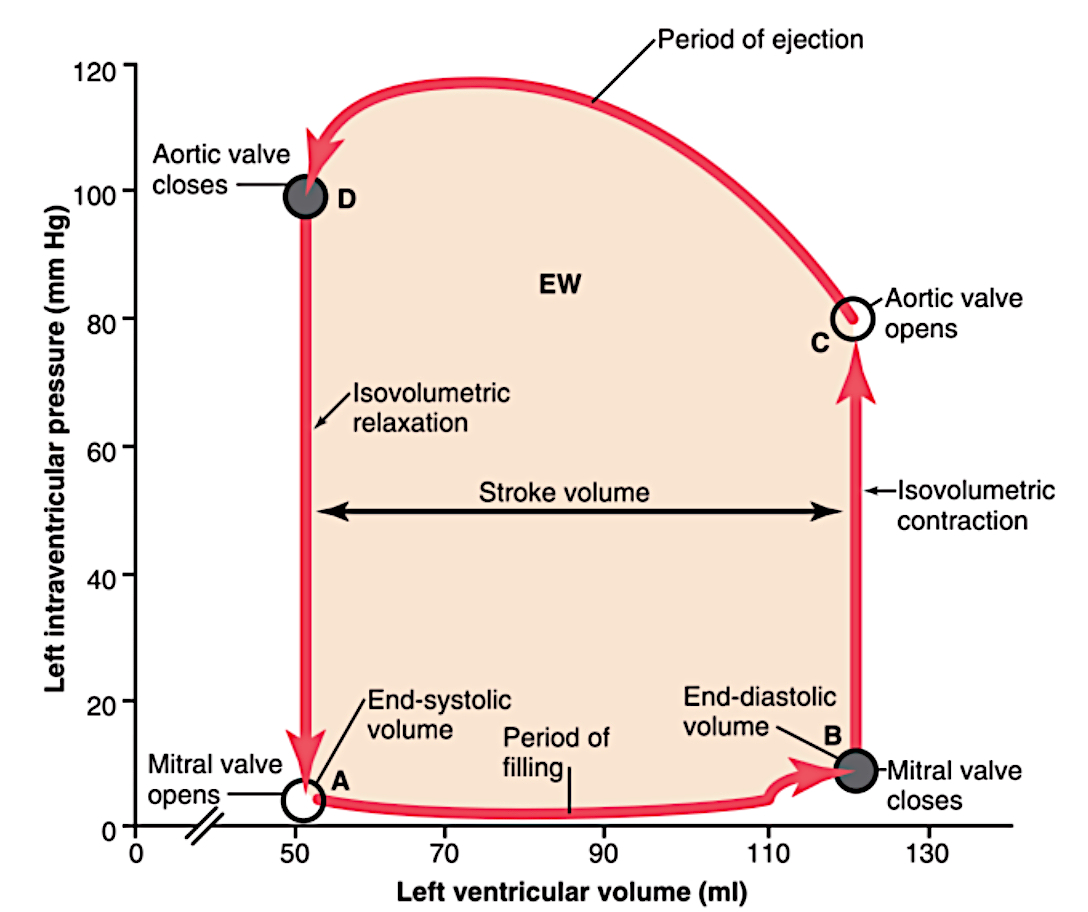
\includegraphics[width=0.5\textwidth]{images/pv_2_.jpg}\label{fig:pv_2}}
  \caption{(a)Working diagram of the left ventricle with the P-V diagram. (b) Close-up P-V diagram. \cite{GH20}}
  \label{fig:pv}
\end{figure}
The blue curve representing the \textit{diastolic pressure} is calculated by gradually filling the heart with higher blood volumes and then measuring the diastolic pressure just before ventricular contraction occurs. It is describing the heart's mechanical properties when the myocardium is in a relaxed state. The green curve in \figurename~\ref{fig:pv_1}, named \textit{systolic pressure}, is plotted by measuring the systolic pressure over varying filling volumes for constant ventricle volumes. The red lines in \figurename~\ref{fig:pv_1} and \figurename~\ref{fig:pv_2} indicate the cardiac cycle and its four action phases, as described above. The line between points A and B in \figurename~\ref{fig:pv_2} depicts the period of rapid filling. The isovolumic contraction is represented through line II in \figurename~\ref{fig:pv_1}, respectively between points B and C in \figurename~ \ref{fig:pv_2}. The ejection phase is represented through III in \figurename~\ref{fig:pv_1} and the line referred to as IV represents the period of isovolumic relaxation. The area of the work diagram, marked with EW in \figurename~\ref{fig:pv} is a measure of the work done by the heart. Knowledge of the P-V diagram is an important prerequisite in understanding myocardial diseases, such as heart failure. \cite{HKS4}

\section{Heart failure}
In the case of heart failure, the heart is unable to provide the required amount of blood flow to the cardiovascular system in order to supply all organs and tissue with oxygen.
Heart failure does not directly represent a disease but rather a clinical syndrome. Nevertheless, the symptoms of different forms of heart failure are very similar and eventually manifest themselves in a decreased cardiac output. One acute consequence of heart failure, for example, is the feeling of shortness of breath. In the long term, however, severe heart failure can also lead to muscle weakness and a lack of concentration.
\\According to \cite{HKS4}, heart failure can be attributed to either systolic dysfunction or diastolic dysfunction. In systolic dysfunction, there is either a limitation of contractility or an impairment of the ejection phase sequence. Causes may include prolonged pressure stress, also called hypertension, or restriction of oxygen supply due to coronary artery disease. Furthermore, cardiac arrhythmias or a heart attack can lead to systolic dysfunction. In diastolic functional impairment, the dysfunction is evident in the course of the filling phase. This can be triggered, among other things, as a result of reduced compliance of the myocardium due to hypertrophy or fibrosis.
\\For the treatment of heart failure, drug therapy using beta-blockers is initially targeted in most cases. However, if this is not successful, the use of ventricular assist devices can be a useful alternative in order to relieve the heart and provide sufficient blood flow. \cite{HKS4}
